\documentclass[a4paper,UTF8]{article}
\usepackage{ctex}
\usepackage{graphicx}
\usepackage{amsmath}
\setCJKfamilyfont{hwxk}{STXingkai}             %使用STXingkai华文行楷字体
\newcommand{\huawenxingkai}{\CJKfamily{hwxk}}
\setCJKfamilyfont{kt}{KaiTi}            % 这里设置是楷体字体 这里可以设置字体
\newcommand{\kaiti}{\CJKfamily{kt}}
\newcommand{\chuhao}{\fontsize{42pt}{\baselineskip}\selectfont}
\newcommand{\sanhao}{\fontsize{15.75pt}{\baselineskip}\selectfont}
\newcommand{\xiaosan}{\fontsize{15pt}{\baselineskip}\selectfont}
\newcommand{\xiaosanp}{\fontsize{13pt}{\baselineskip}\selectfont}
\newcommand{\sihao}{\fontsize{14pt}{\baselineskip}\selectfont} % 这里设置字体大小
\newcommand{\wuhao}{\fontsize{10.5pt}{\baselineskip}\selectfont}
\newcommand{\xiaosi}{\fontsize{12pt}{\baselineskip}\selectfont}
\newcommand{\bt}{\fontsize{16pt}{\baselineskip}\selectfont}
\setCJKmainfont{宋体}
\usepackage{amssymb}
\usepackage{wrapfig}
\usepackage{amsmath}
\usepackage{geometry}
\geometry{a4paper,left=3.17cm,right=3.17cm,top=2.54cm,bottom=2.54cm}
%% 添加首行缩进,两个字符
\RequirePackage{indentfirst}
\setlength{\parindent}{2em}
%% 行距
\setlength{\baselineskip}{20pt}
\selectfont
% 页面顶行空白
\setlength{\topskip}{0ex}
% 段间距
\setlength{\parskip}{1ex}
\renewcommand\figurename{图}
\begin{document}
\newpage
\thispagestyle{empty}% 当前页不显示页码'
\begin{wrapfigure}{l}[0cm]{2pt}
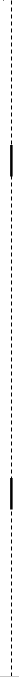
\includegraphics[width=0.3cm,height=29.7cm]{33.png}
\end{wrapfigure}
 ~\\
 ~\\
\center{
\includegraphics[width=5.26cm,height=0.92cm]  {11.jpg}}
 ~\\
 ~\\
 ~\\
 ~\\
\center{\chuhao\huawenxingkai 学\ 生\ 实\ 验\ 报\ 告}\\
\center{\sanhao\huawenxingkai (理工类)}\\
\center{
\includegraphics[width=2.52cm]  {22.png}}
 ~\\
 ~\\
 ~\\
 ~\\
 ~\\
 ~\\
 ~\\
 ~\\
 ~\\
 ~\\
{\heiti {\xiaosanp{课程名称:}\xiaosi\underline{XXXXXXXXXXXXXXXX}\xiaosanp{专业班级:}\xiaosi\underline{1X信安x班}}}\\
~\\
{\heiti {\xiaosanp{学生学号:}\xiaosi\underline{\qquad \ \ 1X120310xx\ \ \ \ \ \ }\xiaosanp{学生姓名:}\xiaosi\underline{\qquad 左XX \qquad }}}\\
~\\
{\heiti {\xiaosanp{所属院部:}\xiaosi\underline{\qquad 软件工程学院\qquad }\xiaosanp{指导老师:}\xiaosi\underline{\qquad XXXX \qquad}}}\\
~\\
 ~\\
\center\textbf\textbf\textbf\sihao\heiti{20 \underline{\ 19\ }\ ——\ 20 \underline{\ 20\ } 学年 \qquad \qquad 第 \underline{\ 2\ }  学期}
 ~\\
~\\
~\\
\center\xiaosi\heiti{金陵科技学院教务处制}
\newpage
\thispagestyle{empty}% 当前页不显示页码'
\begin{flushleft}
~\\
\linespread{1.4}\heiti\textbf\bt {实验报告书写要求}\\
\linespread{1.0}\selectfont\kaiti\xiaosanp{\quad \quad 实验报告原则上要求学生手写,要求书写工整。若因课程特点需打印的,要遵照以下字体、字号、间距等的具体要求。纸张一律采用A4的纸张。}\\
~\\
\linespread{1.4}\heiti\textbf\bt {实验报告书写说明}\\
~\\
\linespread{1.0}\selectfont\kaiti\xiaosanp{\quad \quad 实验报告中一至四项内容为必填项,包括实验目的和要求;实验仪器和设备;实验内容与过程;实验结果与分析。各院部可根据学科特点和实验具体要求增加项目。}\\
~\\
\linespread{1.4}\heiti\textbf\bt {填写注意事项}\\
~\\
\linespread{1.0}\selectfont\kaiti\xiaosanp{\quad \quad (1)细致观察,及时、准确、如实记录。}\\
\linespread{1.0}\selectfont\kaiti\xiaosanp{\quad \quad (2)准确说明,层次清晰。}\\
\linespread{1.0}\selectfont\kaiti\xiaosanp{\quad \quad (3)尽量采用专用术语来说明事物。}\\
\linespread{1.0}\selectfont\kaiti\xiaosanp{\quad \quad (4)外文、符号、公式要准确,应使用统一规定的名词和符号。}\\
\linespread{1.0}\selectfont\kaiti\xiaosanp{\quad \quad (5)应独立完成实验报告的书写,严禁抄袭、复印,一经发现,以零分论处。}\\
~\\
\linespread{1.4}\heiti\textbf\bt {实验报告批改说明}\\
~\\
\linespread{1.0}\selectfont\kaiti\xiaosanp{\quad \quad 实验报告的批改要及时、认真、仔细,一律用红色笔批改。实验报告的批改成绩采用百分制,具体评分标准由各院部自行制定。}\\
~\\
\linespread{1.4}\heiti\textbf\bt {实验报告装订要求}\\
~\\
\linespread{1.0}\selectfont\kaiti\xiaosanp{\quad \quad 实验批改完毕后,任课老师将每门课程的每个实验项目的实验报告以自然班为单位、按学号升序排列,装订成册,并附上一份该门课程的实验大纲。}\\
\end{flushleft}
\newpage
\thispagestyle{empty}% 当前页不显示页码'
\begin{flushleft}
\linespread{1}{\heiti {\sihao{实验项目名称:}\sihao\underline{XXXXXXXXXXXXXXXXXXXXXXXXX}\sihao{实验学时:}\sihao\underline{2课时}}}\\
\linespread{1}{\heiti {\sihao{同组学生姓名:}\sihao\underline{\qquad \qquad }\sihao{实验地点:}\sihao\underline{\qquad \qquad \qquad}}}\\
\linespread{1}{\heiti {\sihao{实验日期:}\sihao\underline{\qquad \qquad \qquad}\sihao{实验成绩:}\sihao\underline{\qquad \qquad \qquad}}}\\
\linespread{1}{\heiti {\sihao{批改教师:}\sihao\underline{\quad \  XXXX \ \quad}\sihao{批改时间:}\sihao\underline{\qquad \qquad \qquad}}}\\
\end{flushleft}
\newpage
\thispagestyle{empty}% 当前页不显示页码'
\begin{flushleft}
\heiti\sihao {一、实验目的和要求}\\
\end{flushleft}
\begin{figure}[htb] 
 \center{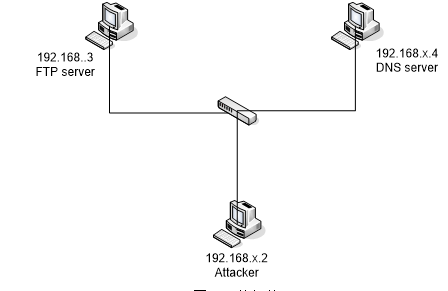
\includegraphics[width=11.4cm,height=7.30cm]  {19.png}} 
 \caption{这是插入了一张悬浮图} 
\end{figure}
\begin{flushleft}
\heiti\sihao {二、实验仪器和设备}\\
{{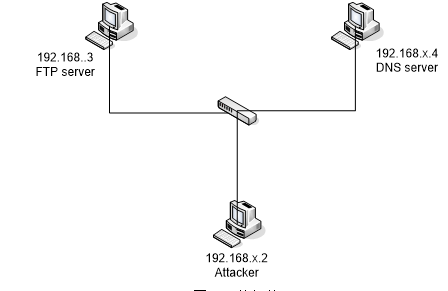
\includegraphics[width=11.4cm,height=7.30cm]  {19.png}}\\\songti\wuhao{图4 这里添加了一个普通的照片} }\\
\heiti\sihao {三、实验内容与过程}\\

\linespread{1.0}\selectfont\songti\wuhao{\quad \quad 这里我们在查看目标主机的arp表,我们发现攻击机分别在两台主机上充当了另一方,成为了这个网络的中间人,这也表示攻击成功}\\
~\\
~\\
~\\
~\\
\heiti\sihao {四、实验结果与分析 一级标题}\\
\linespread{1.0}\selectfont\heiti\xiaosi {4.1 二级标题}\\
~\\
~\\
~\\
~\\
\heiti\sihao {五、思考题}\\
~\\
~\\
~\\
~\\
~\\
\heiti\sihao {六、实验心得}\\
~\\
~\\
~\\
~\\
\end{flushleft}
\end{document}


% 这一部分是插入图片
% 这是插入悬浮图片
%\end{flushleft}
%\begin{figure}[htb] 
% \center{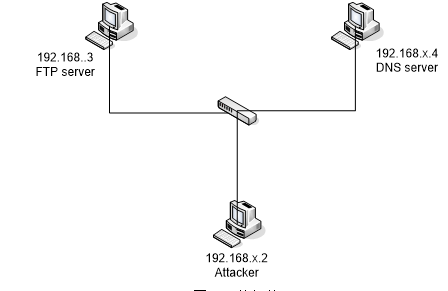
\includegraphics[width=11.4cm,height=7.30cm]  {19.png}}  %这里设置图片长宽,还有图片(这里的图片存放在tex文件的根目录)
% \caption{网络拓扑} %这里设置图注的名字
%\end{figure}
%\begin{flushleft}
% 这里插入普通图片
% \center{{\includegraphics[width=15.85cm,height=3.48cm]  {20.png}}\\\songti\wuhao{图4 192.168.x.2主机中wireshark抓取的ICMP数据包} } 这里还是和这个一样的

% \begin{flushleft}
% \heiti\sihao {六、实验心得}\\ %这里是插入一个四号黑体的标题
% \linespread{1.0}\selectfont\heiti\xiaosi {4.1 利用工具cain进行ARP欺骗}\\
% \linespread{1.0}\selectfont\kaiti\xiaosanp{\quad \quad (1)细致观察,及时、准确、如实记录。}\\ 这里是插入了行距为1.0倍,楷体小四号修改后的段落
% \linespread{1.4}\heiti\textbf\bt {实验报告书写要求}\\ %这里是插入了行距1.4倍黑体加粗的标题
% \linespread{1.0}\selectfont\songti\sihao{\quad \quad(1)1台攻击机,IP地址为192.168.x.2,安装软件为cain.exe\\ \quad \quad(2)2台靶机,IP地址分别为192.168.x.3、192.168.x.4\\ \quad \quad(3)192.168.x.3上安装了FTP服务器,用户名为administrator,口令为Simplexue123。\\ \quad \quad(4)192.168.x.4上配置了DNS服务器。}\\ 这里插入了一个1.0倍行距宋体四号的段落
% \end{flushleft}

% 这是反斜杠 $\backslash$ \_ 这是下划线

% \newpage
% \thispagestyle{empty}% 当前页不显示页码'
% 这里是为了新建一页顺便设置当前页面不使用页码 

% \\ 换行 ~\\空一行
% \[ ] 小空格 \quad 大空格 \qquad 超大空格




